\documentclass[eng]{class}
% Publication Title
\title{Video curriculum : Something about me}
% Short title for the header (copy the main title if it is not too long)
\shorttitle{Something about me}
       
% Authors
\author{D. Ligari 518592}
% Author Affiliations
\affil{Digital content retrieval, University of Pavia, Department of Computer Engineering (Data Science), Pavia, Italy}
% Surname of the first author of the manuscript
\videolink{https://youtu.be/NYCtO0WvBkE}
\firstauthor{D. Ligari}
%Contact Author Information
\contactauthor{D. Ligari} % Name and surname of the contact author
\email{davide.ligari01@universitadipavia.it} % Contact Author Email
% Publication data (will be defined in the edition)
\publicationdate{\today}
% Place your particular definitions here
\newcommand{\vect}[1]{\mathbf{#1}}  % vectors

\abstract{ This project focused on editing and organizing a videocurriculum as a real world project.
 A Work Breakdown Structure (WBS), Gantt chart,SWOT and risk analysis were utilized for effective management. 
 The WBS provided a hierarchical breakdown of tasks, facilitating coordination. The Gantt chart aided in scheduling, 
 resource allocation, and progress monitoring. 
 The risk analysis identified and mitigated potential threats. 
 By implementing these techniques, the project achieved efficiency and successful completion. 
 This report presents a systematic approach for managing similar complex projects, offering valuable insights for future endeavors.}
\keywords{ Video curriculum • Project management • WBS • GANTT • SWOT • Risk analysis}
\date{\today}
% Start document
\begin{document}
% Include title, authors, abstract, etc.
\maketitle
\tableofcontents
\thispagestyle{FirstPage}
%Figures and tables must be cited in the text and explained in detail. Do not forget to add a caption to each figure/table/
\section{Introduction}
\firstword{I}{n}
today's fast-paced and technologically driven world, the demand for innovative and engaging way to share the personal and working experiences has grown exponentially.
Traditional forms are increasingly being supplemented or even replaced by digital resources that leverage the power of multimedia.
Among these resources, video curriculum have emerged as a popular and effective alternative to the traditional curriculum.\\
A video curriculum is a short video that provides a concise overview of a person's professional and educational background.
The creation and management of a video curriculum, however, present unique challenges.
It requires meticulous planning, organization, and project management skills to ensure the seamless editing and effective organization of the video content.
Treating a video curriculum project as a complex endeavor can greatly enhance its success by providing a structured framework for its development.\\
This report focuses on the project management aspects of editing and organizing a video curriculum as if it were a real complex project.
It emphasizes the importance of employing project management techniques such as a Work Breakdown Structure (WBS), a Gantt chart,
a SWOT and a risk analysis to ensure efficient execution and successful completion. By adopting these techniques,
i can effectively navigate the complexities inherent in video curriculum development,
resulting in a high-quality resource that meets the needs of recruiters.
\section{Work Breakdown Structure (WBS)}
\pagestyle{OtherPage}
\begin{figure}[b!]
  \centering
  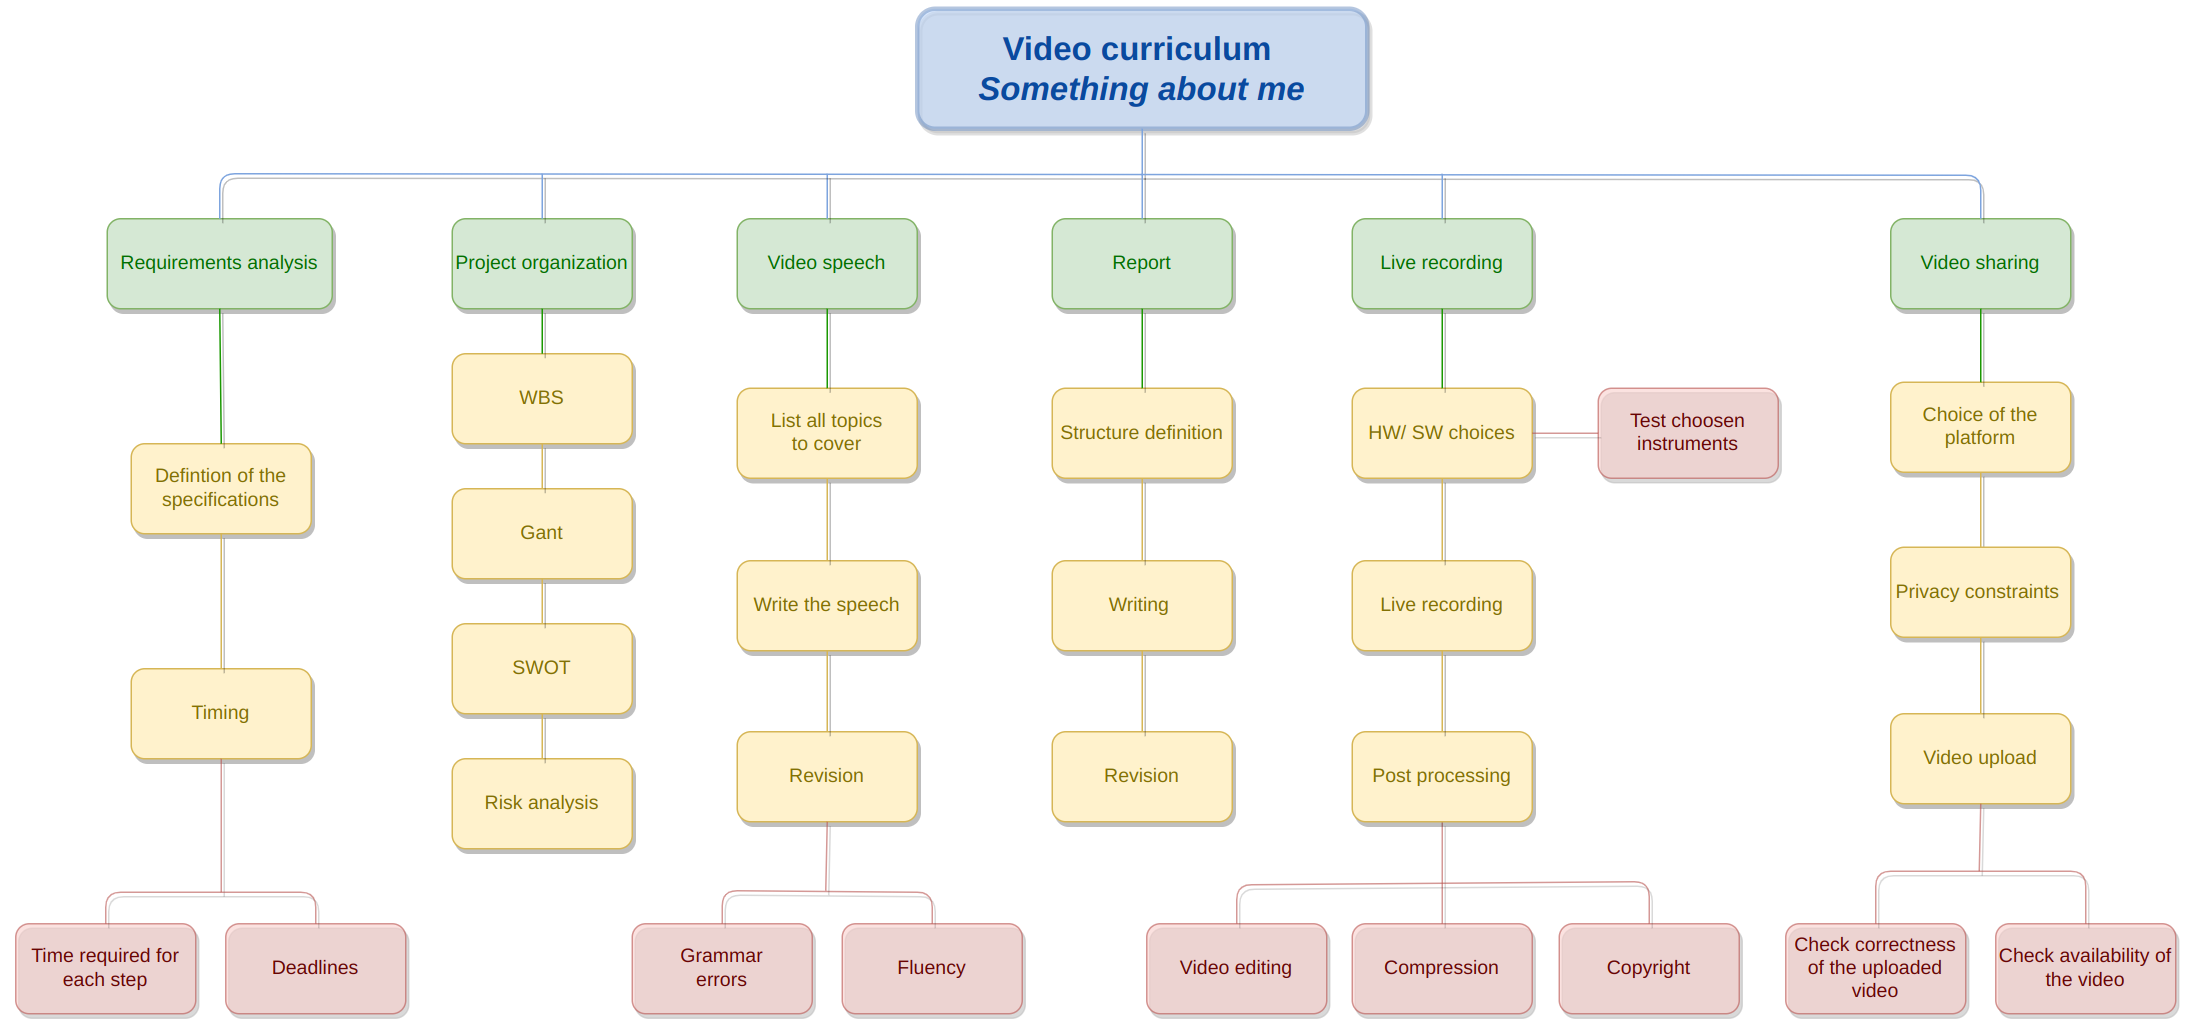
\includegraphics[width=\textwidth]{images/wbs.png}
  \caption{WBS of the project}
  \label{fig-1}
\end{figure}
The Work Breakdown Structure (WBS) is a fundamental project management tool that provides a hierarchical breakdown of tasks and deliverables within a project.
In the context of video curriculum editing and organization, the WBS serves as a roadmap,
delineating the various activities and subtasks involved in the project's execution.
By breaking down the project into manageable components, the WBS enables effective coordination, resource allocation, and task management.\\
There are several types of WBS, including the deliverable-based, phase-based, and hybrid WBS.
In this project, a phase-based WBS was utilized, as it is the most commonly used and intuitive type, because it organizes tasks according to the  phases or stages of the project.
It provides a high-level overview of the project's progression and helps in managing tasks sequentially.\\
The Work Breakdown Structure (WBS) of the project, depicted in Figure 1, was organized into three levels.
Level 1 (green) represents the macro phases of the project, Level 2 (yellow) comprises the activities, and Level 3 (red) encompasses the sub-activities.
The project phases were arranged in a temporal sequence to facilitate effective management of the activities.
The project consisted of six macro-phases:\\
\\
\textbf{Requirement Analysis:}\\
This phase involved identifying the specifications imposed by the teacher for the video curriculum.
Additionally, deadlines for delivery (17 June) and timelines for each project phase were established.\\
\\
\textbf{Project Organization:}\\
During this phase, essential project management documents, including the WBS, GANTT chart, SWOT analysis, and risk analysis, were drafted.\\
\\
\textbf{Video Speech:}\\ This phase encompassed selecting topics to be covered in the video curriculum and preparing the speech to be delivered.
Corrections of pronunciation and grammatical errors were addressed.\\
\\
\textbf{Report:}\\ The report phase involved defining the general structure, topics, and relevant sections of the report.
This was followed by drafting the report and conducting a final revision.\\
\\
\textbf{Video Sharing:}\\
During this phase, video sharing platforms were analyzed, considering privacy concerns,
as the decision was made not to make the video curriculum public. The most suitable platform was chosen for sharing the video curriculum,
which underwent a final review before completion.
\clearpage
\section{GANTT Chart}
\begin{figure}[b!]
  \centering
  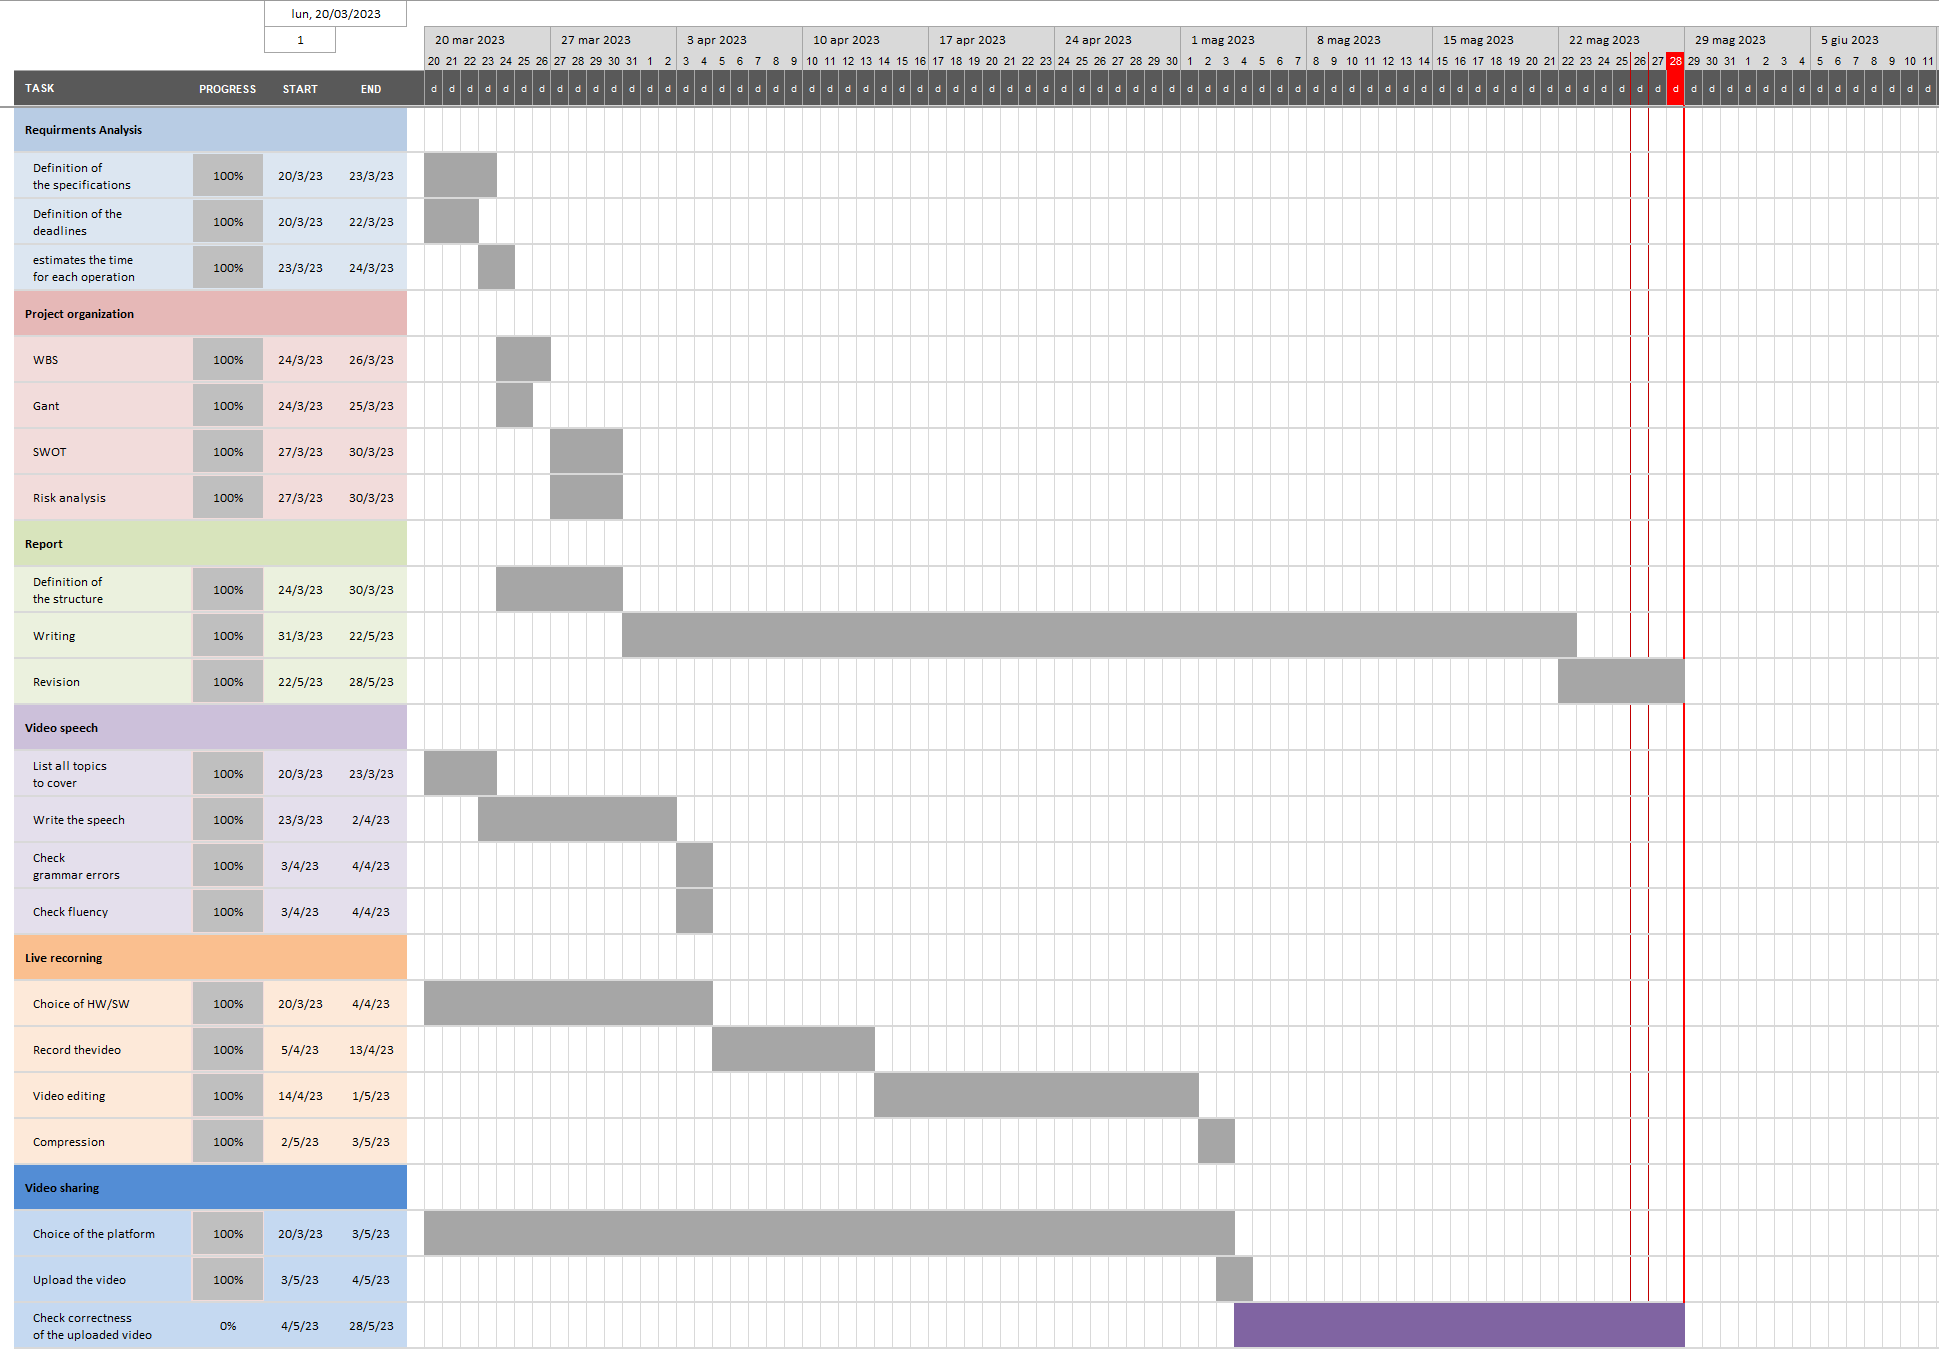
\includegraphics[width=0.9\textwidth]{images/gantt.png}
  \caption{Gantt chart}
  \label{fig-2}
\end{figure}
The Gantt chart is a widely adopted project management tool that provides a visual representation of project tasks, timelines, and dependencies.\\
In the context of the video curriculum editing and organization project, the Gantt chart played a critical role in planning, scheduling,
and monitoring project progress. By visually illustrating the project timeline and task interdependencies, the Gantt chart facilitated effective coordination,
resource allocation, and timely execution of project activities.
Figure \ref{fig-2} presents the  Gantt chart, which served as a visual representation of the project's timeline and activities.
Each phase of the project was further divided into sub-phases, allowing for a granular breakdown of tasks and deliverables.\\
A key aspect of developing the Gantt chart was to ensure the seamless coordination of activities by respecting
the dependencies between the various sub-phases.
For instance, the video recording phase was scheduled to commence only after the text had been written and corrected.
This approach aimed to streamline the workflow and promote efficient task progression, maximizing productivity and minimizing potential bottlenecks.\\
To provide a buffer for unforeseen challenges and potential delays, the deadline was set to 28 May.
This buffer period allowed for the mitigation of risks and provided an additional timeframe for addressing any unexpected obstacles that might arise.\\

\section{SWOT Analysis}
The SWOT analysis is a widely used strategic planning tool that helps organizations assess their internal strengths and weaknesses,
as well as external opportunities and threats. It provides a comprehensive framework for evaluating the current state of an organization or a project,
identifying areas of advantage and areas that require improvement, and uncovering potential opportunities and challenges in the external environment.\\
SWOT is an acronym that stands for Strengths, Weaknesses, Opportunities, and Threats. Strengths and weaknesses refer to internal factors within the organization,
such as resources, capabilities, processes, and performance.
\clearpage
\noindent
Opportunities and threats, on the other hand, are external factors that arise from the
business environment, market trends,
competition, or regulatory changes.
\begin{figure}[t!]
  \centering
  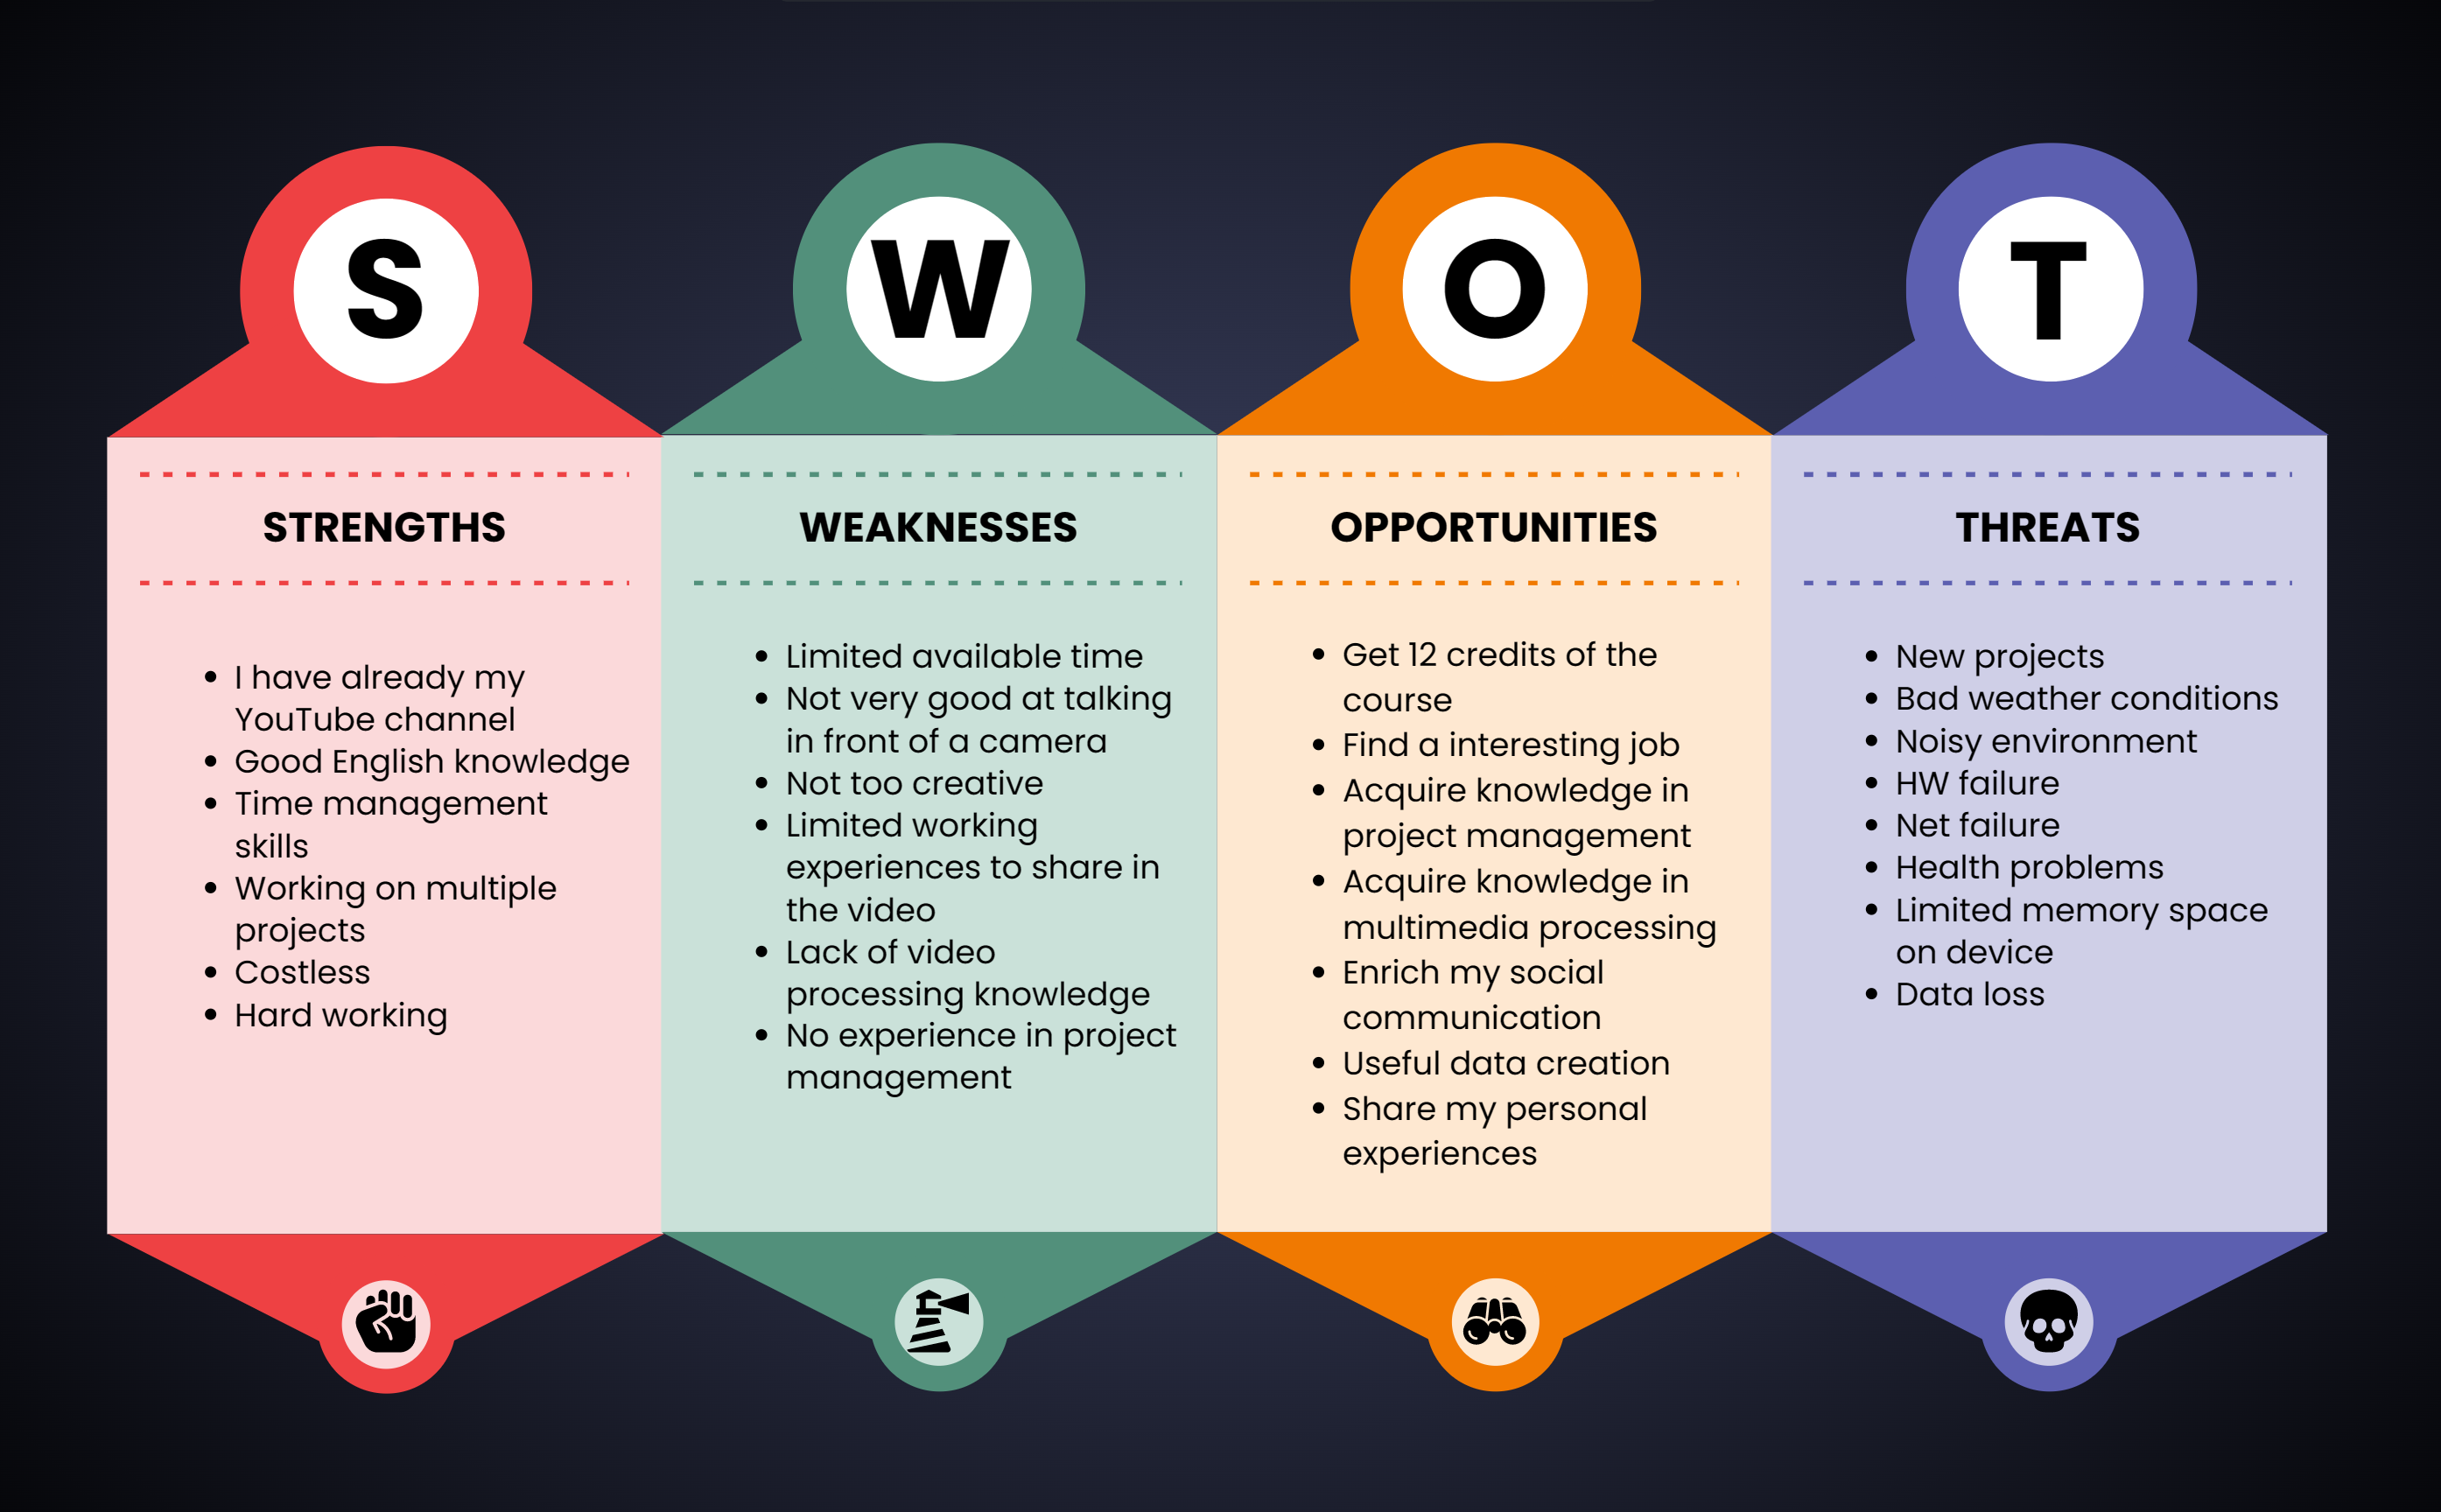
\includegraphics[width=\textwidth]{images/SWOT.png}
  \caption{SWOT analysis}
  \label{fig-3}
\end{figure}
\noindent
The purpose of conducting a SWOT analysis is to gain a deeper understanding of the organization's position,
make informed decisions, and develop strategies that leverage strengths, mitigate weaknesses, capitalize on opportunities,
and mitigate threats. By systematically evaluating these four dimensions, organizations can align their resources and efforts to achieve their
objectives and navigate through dynamic and competitive landscapes.\\
Figure \ref{fig-3} presents the SWOT analysis of the video curriculum project.

\section{Risk Analysis}
In any project, regardless of its nature or complexity, the presence of uncertainties and potential risks is inevitable.
These risks can arise from various sources, such as technical challenges, resource limitations, external factors, or unforeseen events.
To ensure successful project outcomes, it is crucial to proactively identify, assess, and mitigate these risks. This is where risk analysis plays a vital role.\\
Risk analysis is a systematic process that involves identifying potential risks, evaluating their probability of occurrence and potential impact,
and
\\
\\
\\
\\
\\
\\
\\
\\
\\
\\
\\
\\
\\
\\
\\
\\
\\
\\
\\
\\
\\
\\
\\
\\
\\
developing strategies to mitigate or manage them effectively. By conducting a comprehensive risk analysis,
i can enhance my understanding of the project's vulnerabilities and proactively address potential obstacles that may impede progress or success.\\
\subsection{Negative risks}
In any project, there are inherent uncertainties and potential events that may have adverse effects on its successful completion.
These events, commonly referred to as risks, can range from unexpected obstacles to external factors beyond the my control.
It is crucial to identify and assess these negative risks proactively to develop appropriate strategies for their mitigation or contingency.
Negative risk analysis is a systematic approach that aims to identify, evaluate, and manage potential risks that may impact the project's objectives negatively.
This analysis focuses on anticipating and addressing potential threats to minimize their potential negative consequences.\\
For each identified risk, a comprehensive assessment was conducted to determine both its probability of occurrence and the potential impact it could have on the project.
By quantifying the likelihood and magnitude of the risks, i could effectively allocate resources and develop mitigation strategies accordingly.\\
Figure \ref{fig-4} provides a graphical representation of the negative risk analysis conducted for the project.
It showcases the identified risks along with their associated probability, impact levels and actions that can be taken to prevent or solve it. This visual analysis served as
a valuable tool to gain a comprehensive understanding of the risk landscape and prioritize their efforts
in risk mitigation and contingency planning.
\begin{figure}[h!]
  \centering
  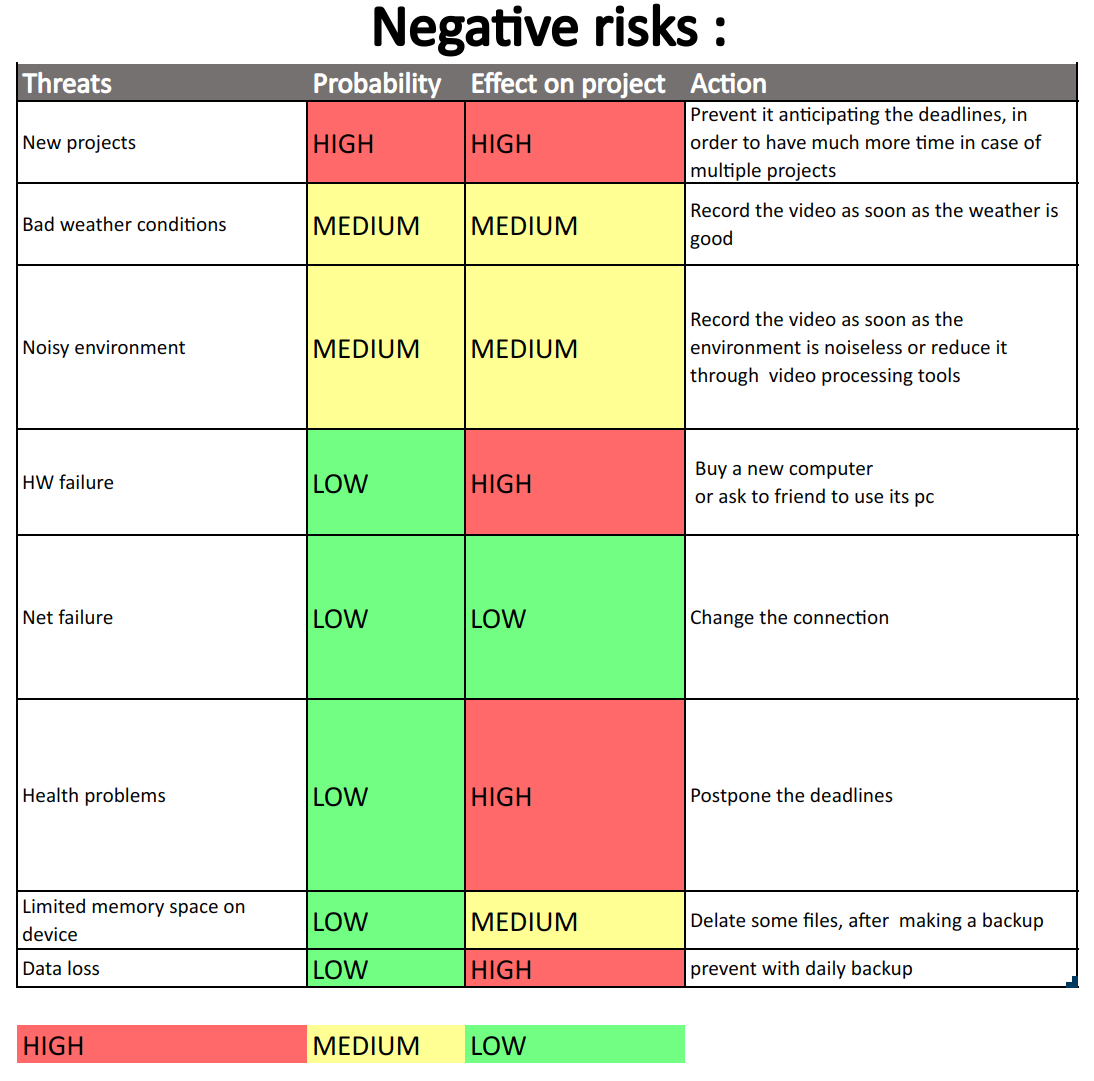
\includegraphics[width=\columnwidth]{images/negative risks.png}
  \caption{Negative risk analysis}
  \label{fig-4}
\end{figure}


\subsection{Positive risks}
While risks are often associated with negative outcomes, it is important to recognize that not all risks are detrimental.
Positive risks, also known as opportunities, present favorable circumstances that can lead to project enhancements, improved outcomes, and increased value.
Conducting a positive risk analysis allows the identification and capitalization on these opportunities, maximizing the project's potential for success.\\
An analysis was conducted not only for negative risks but also for positive risks, aiming to assess their probability of occurrence,
potential impact on the project, and identify actions to maximize their benefits (Figure \ref{fig-5}).
By proactively addressing positive risks, is possible to exploit opportunities that could enhance project outcomes.
The analysis provided insights into the likelihood of positive events, their potential influence, and enabled the formulation of strategies to
capitalize on them effectively.
\begin{figure}[h!]
  \centering
  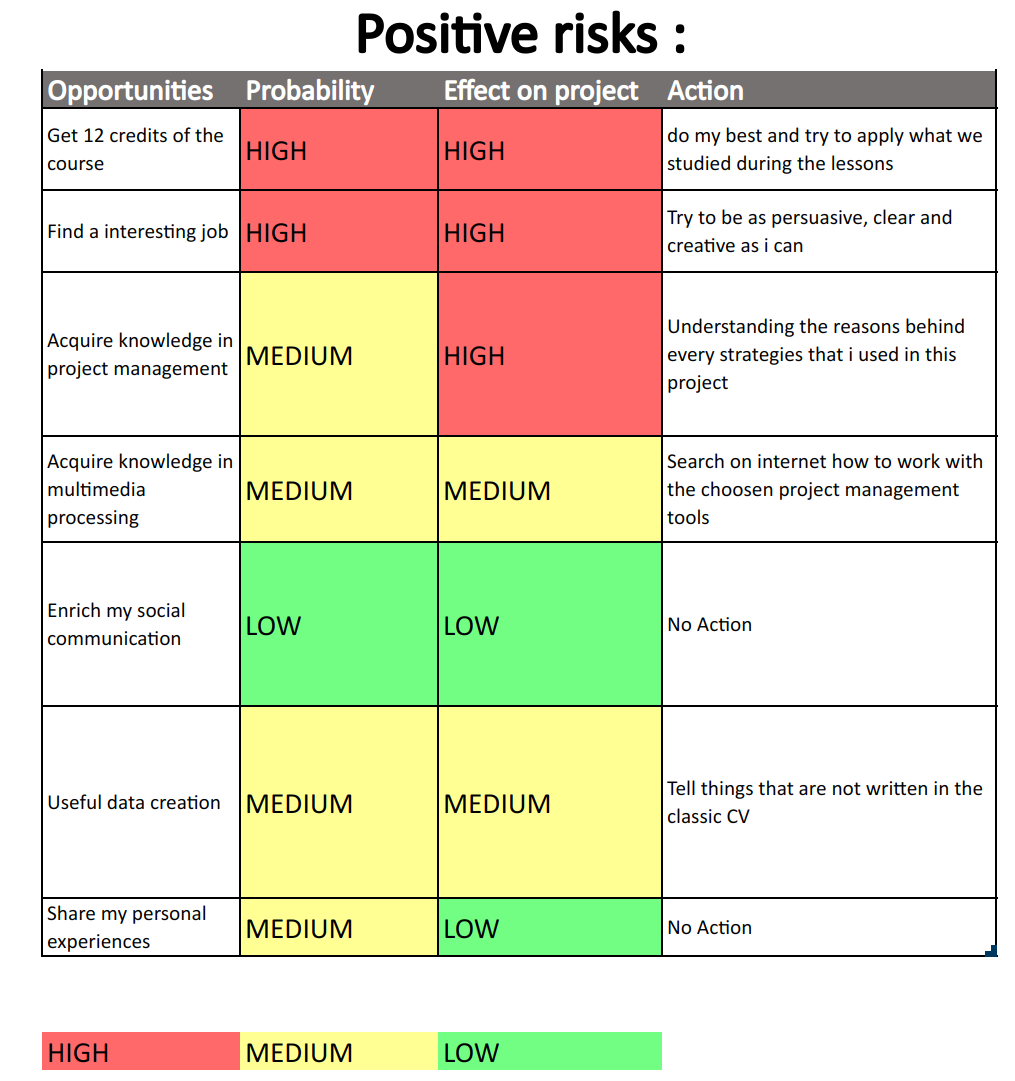
\includegraphics[width=\columnwidth]{images/positive risks.png}
  \caption{Positive risk analysis}
  \label{fig-5}
\end{figure}

\section{Video creation and editing}
The video was captured using an iPhone 13, utilizing its 4K resolution and 60 frames per second (fps) capability to ensure high-quality footage.
Multiple video clips were shot and later merged and edited using Filmora video editing software for seamless transitions and desired visual effects.\\
To optimize the video for streaming purposes, it was exported in MP4 format at a resolution of 1080 and 25 fps, striking a balance between quality and file size.\\
The language chosen for the video is English, which is deemed more appropriate considering the data science course is taught in English.
Additionally, English is widely recognized as the global language of communication in the professional world, and its importance is growing even in Italy.
Consequently, a video curriculum presented in English has the potential to leave a lasting impression on recruiters, highlighting the candidate's proficiency
in a language that holds significant value in today's global job market.\\
It is worth noting that all media files used in the video were obtained from reputable sources that provide free and non-copyrighted content.
However, it is important to mention that the background music used in the video has certain usage restrictions.
It cannot be sold or distributed as a standalone product in either digital or physical form, and care was taken to ensure
it is not used in a misleading or deceptive manner.\\
YouTube was selected as the ideal platform for sharing the video curriculum, given its widespread popularity as the leading video-sharing platform.
Additionally, YouTube provides convenient privacy settings, allowing the video to be set as private, ensuring that only individuals with the link can access it.
This feature ensures controlled access and enhances confidentiality for the intended audience.\\
To ensure the safety and preservation of all project files, a backup copy of the video curriculum and associated files was uploaded to OneDrive.
This cloud-based storage solution offers a reliable and secure platform for storing and accessing project files from any location,
providing peace of mind in case of data loss or unforeseen technical issues.\\
\section{Conclusions}
In conclusion, the completion of this project highlights
the significance of effective project management and adaptability when faced with challenges.\\
Despite encountering delays during the video recording phase due to a lack of experience and difficulties in the editing phase with the software,
the project was successfully accomplished within the imposed deadlines.



\end{document}